\documentclass[letterpaper,10pt,serif,draftclsnofoot,onecolumn,compsoc,titlepage]{IEEEtran}

\usepackage{graphicx}                                        
\usepackage{amssymb}                                         
\usepackage{amsmath}                                         
\usepackage{amsthm}                                          
\usepackage{cite}
%\addbibresource{SpMPR\_Group51.bib}
\usepackage{alltt}                                           
\usepackage{float}
\usepackage{color}
\usepackage[hyphens]{url}
\usepackage{pgfgantt}
\usepackage{rotating}
\usepackage{enumitem}
\usepackage{gensymb}
\usepackage[T1]{fontenc}

\usepackage{balance}
\usepackage[TABBOTCAP, tight]{subfigure}
\usepackage{enumitem}

\usepackage{geometry}
\geometry{margin=.75in}
\usepackage{hyperref}
\usepackage{breakurl}
%\usetikzlibrary{shapes, positioning, calc}
\usepackage{caption}
%\usepackage[utf8]{inputenc}
%pull in the necessary preamble matter for pygments output

\definecolor{dkgreen}{rgb}{0,0.6,0}
\definecolor{gray}{rgb}{0.5,0.5,0.5}
\definecolor{mauve}{rgb}{0.58,0,0.82}

\usepackage{listings}
\lstset{
  frame=single,
  language=C,
  basicstyle=\small,
}

%% The following metadata will show up in the PDF properties
\hypersetup{
   colorlinks = true,
   citecolor = black,
   linkcolor = black,
   urlcolor = black,
   breaklinks = true,
   pdfauthor = {Shu-Ping Chien, Brock Smedley, W Keith Striby Jr},
   pdfkeywords = {CS463 "Senior Project" Progress Report},
   pdftitle = {CS463 Spring Midterm Progress Report},
   pdfsubject = {CS463 Spring Midterm Progress Report},
   pdfpagemode = UseNone
}

\parindent = 0.0 in
\parskip = 0.1 in
\title{Winter Midterm Progress Report: Multi-Camera, SoM Based, Real-Time Video Processing for UAS and VR/AR Applications}
\author{Area 51: Shu-Ping Chien, Brock Smedley, W Keith Striby Jr \\ 06 May 2018 \\ CS463, Senior Software Engineering Project, Spring 2018}


\begin{document}
\begin{titlepage}
\maketitle

\begin{abstract}

This document highlights the group's progress made during the first half of the 
Spring 2018 term. The project is introduced along with an explanation of the 
hardware and software surrounding our product's planned solution. \\

EDIT THIS:\\
Then each group member
explains their contributions to the project, what they have remaining to complete
the projects requirements, and problems experienced with solutions if applicable. \\


\thispagestyle{empty}
\end{abstract}
\end{titlepage}

\newpage
\tableofcontents

\newpage

\section{Introduction}

\subsection{Purpose}
Our project is required to provide a video output at near real-time from a 
multi-camera input utilizing an NVIDIA Jetson TX1 or TX2 system-on-module (SoM). 
The software produced will perform image processing and edge computing on the 
camera input to display a visually enhanced and stitched video output. 
Size, weight, power, and cost (SWaP-C) requirements for the project are due 
to its application being for UAS and VR/AR, and from our system utilizing a 
mass-produced SoM, particularly the Jetson TX2. \\

\subsection{Scope}

Application specific hardware and software are vital for the project due the the 
system requirements and constraints of the project.
The NVIDIA Jetson TX2 runs on an Ubuntu based Linux for Tegra (L4T) operating 
system created specifically for producing customized imaging, installed on a 
GPU-accelerated dual-core CPU with dual Image Signal Processors (ISPs). \\

L4T, being an Ubuntu variant, provides a friendly development interface with 
access to a large repository of additional software. NVIDIA provides the Jetson 
Software Development Pack (JetPack) 3.1 which has L4T 28.1 
and is capable of supporting a multitude of multimedia and image processing 
application program interfaces (APIs). Jetpack 
is installed on an Ubuntu host computer and is then flashed to the TX2's memory, and 
selected libraries are then installed when the TX2 is self-sustaining. \\

The cameras will utilize the most widely used camera interface for mobile applications, 
MIPI CSI-2, which is capable of supporting 1080p, 4k, and 8k video. 
A carrier board will connect the cameras to the Jetson TX2 that also provides 
additional application-specific interfaces and peripherals. \\

The software materials for this project will support the NVIDIA Jetson TX2 and 
be able to produce stitched images from cameras in near real-time. The data input 
from cameras are sent through the CSI and carrier board, and then arrive at our 
software in the TX2 in raw pixel form. The pixels are then processed through our 
GStreamer pipelines for distributing and transforming their data to the image 
processor. OpenCV libraries in our software is used to access the data in the image 
processor to produce our desired image output. Due to 
using CSI cameras the process avoids writing to memory and 
therefore reading our input data to storage which reduces latency. The image processing 
software will utilize the images from media stream and produce a streaming video 
to the display device.  \\

\subsection{Overview}

This document provides a recap of the progress made on our project through the first half
of the Spring 2018 term. This term the group has been focused on getting rid of our 
issues surrounding latency when streaming video before and after image processing. 
For our current project status we discuss what we have done to test and troubleshoot 
latency, the capabilities of our image processing, and testing performed so far. 
Then the work remaining for the project is elaborated on, which focuses on more 
troubleshooting of our latency issues and finishing testing of our product. Then we will 
discuss problems experienced and solutions where applicable. Finally the report concludes 
with our three-camera GStreamer pipeline code and images of our software output. \\

\section{Current Project Status}

intro\\

\subsection{Image Processing}

types\\

\subsection{Testing}

stuff\\

\subsection{Troubleshooting Latency}

stuff\\

\subsubsection{GStreamer research}

stuff\\

\subsubsection{TX2 Rebuild}

Due to the loosely structured nature of non-versioned project collaboration, our 
first TX2 system build was a bit unstable. To resolve any system configuration errors 
and ensure that the new build was properly configured, the team decided to procure 
another TX2 and rebuild it from scratch. In order to do this reliably, the team 
dedicated one member to build the new system and document the details in order to 
verify 1. That the system wasn't causing issues with our stitching software, and 2. 
That we could reliably rebuild a working module without any system errors.\\

The first part was the simplest to verify: once the new build was completed, we 
tested the new module against our image processing software and verified that the 
problem did in fact lie within our implementation, and not in the system 
configuration. The second part, documenting the process, was also very simple. Bash 
scripts can be used to automate a large portion of the build process, including 
launching Jetpack, flashing the module with the Spacely board support image, and 
installing software libraries on the newly-installed operating system. We simply 
copied the commands which we originally used to build the platform into an executable 
file, which we then could run with one simple command.\\

\section{Work Remaining for Project}
%Describe what you have left to do \\

In the remaining weeks that we have to work on the software of our project we hope to 
solve the latency in our GStreamer pipeline and image processing. Questions surrounding 
our existing pipelines will continued to be asked and therefore adjusted. If our 
troubleshooting fails or after the hopeful success of fixing it, we will complete latency 
and frame rate testing of our software. This section elaborates on our plan of attack to 
complete these tasks.\\

\subsection{Troubleshooting Latency}

Although we have scoured the internet in search of solutions to our latency issues we must 
continue this effort until we are no longer allowed to. Troubleshooting has isolated the 
issue in two areas, the first being our GStreamer pipelines, and the second being during 
image processing. This is how our troubleshooting will continue to be isolated and attacked, 
and this will continue until further isolation is determined or if our software requires 
any major overhaul. \\

In GStreamer pipelines commands are noted with the exclamation mark, and these denote 
filters or pads. The pipelines in our software have several of these pads to mutate 
the input coming from the cameras so the data ready for image processing. We are continuing 
to tinker with and manipulate our pads to see if there is any change in system response. \\

Research surrounding more solutions to our GStreamer latency has not turned up much 
due to the lack of elaboration we are able to find. Resources on GStreamer tend to show 
only examples with limited explanation, making it difficult for us to determine where 
our issue is. Our search for answers will continue looking for resources elaborating on 
GStreamer pipelines. \\

Latency surrounding our image processing software will be sought after when we solve the 
issue of our GStreamer pipelines. We are unable to determine the effect our latency has 
on image processing of stitched and tiled videos and therefore would be an ineffective 
use of our time. Solutions have been found regarding our slow image processing but not 
implemented, and we will determine what path to take when our GStreamer latency issues 
are solved based on how much latency remains, if any. \\

\subsection{Finish Latency and Frame Rate Tests}

The completion of our latency testing has been delayed in hopes of finding a solution to 
the latency in our GStreamer pipeline. Since we know and understand the amount of latency 
that exists in the GStreamer pipeline all that is remaining is determining the amount of 
latency in our stitching and tiling software. \\

Our latency tests are fairly simple to setup and perform. With the software running and 
producing a video output, a running stop-watch is placed on the output screen in a window 
next to it. With the cameras pointed at the output screen showing the stop-watch we then 
take a picture of these two windows side-by-side. The difference in time captured in our 
picture shows the amount of latency between the stop-watch in real-time and following 
image processing. \\

Accompanied with our latency tests we have decided to also produce frame rate testing for 
our client. The frame rate of our software was questioned during the troubleshooting of 
our latency issues, and since frame rate is part of our GStreamer pipeline it is easily 
adjusted and displayed on the output display. This test has been performed with a two and 
three-camera setup of our GStreamer output and produces the expected result of 30 frames 
per second.  \\

\section{Problems Experienced and Solutions (if applicable)}
%Describe any problems that have impeded your progress, with any solutions \\

This section details the various problems we have encountered during the course of development, 
and our attempts and ideas about solutions to these problems.

\subsection{Latency in our Image Processing}
Our image processing software, namely our "stitching" program, which combines two overlapping 
images into one wider image, suffers from high latency and low frame rate. The team has 
identified three potential culprits:

\paragraph*{GStreamer} It is possible that GStreamer is incapable of processing the camera 
data at the bandwidth required to produce a fair-quality image (1280x720) at a reasonable frame 
rate ($\ge$24 fps). Although GStreamer is a widely-used image-processing software, and should be 
able to handle the bandwidth, we have not had the chance to look into alternatives until recently. 
OpenCV allows for the use of Video4Linux, but since we only had one working build, we decided not 
to test an alternate configuration for fear of ruining our only working version. We also have the 
option of using libargus instead of GStreamer, and there is also the option to run a native V4L2 
application (which appears to offer the lowest latency by way of structure) 
[see TX2 architecture figure].

\paragraph*{nvcamerasrc} A GStreamer plugin which is designed to deliver the video stream to our 
image-processing software, may not be suitable for high-bandwidth processing. nvcamerasrc offers 
Image Signal Processor control, which allows us to adjust cameras for lighting and color conditions, 
so it does seem useful, but there are other options available. In [this figure] we see alternatives 
like v4l2src, which is also a GStreamer plugin. v4l2src connects directly to the V4L Mediacontroller 
(bypassing the "Camera Core" software layer), and libargus, which is completely separate from GStreamer.

\paragraph*{OpenCV Stitcher} It is possible that our implementation of the OpenCV Stitcher class may 
be less-than-optimal. While the group did program it to use the GPU (which should be the fastest), 
there are still a lot of moving parts, so to speak, that could be inhibiting the system's performance. 
In the official OpenCV 3.3 documentation \cite{Stitcher}, there is a "mode" option that specifies 
whether to use a 'panorama' or a 'scan.' According to the documentation, panoramas, which we currently 
use, are best used for photographic panoramas. The 'scan' option uses an Affine Transformation 
algorithm, which may offer better performance. OpenCV Stitcher also allows for fine-tuned control, 
as described in the documentation.

\subsection{TX2 Rebuild}
Rebuilding the TX2 was an arduous task. Our original system, as mentioned previously, was built 
collaboratively, with all changes being recorded into a Google Doc. In order to build a new, 
reliable system, we had to pore through our progress document (which grew to ~30 pages) and cipher 
out which bits were needed and which were not. Unfortunately, some software conflicts arose 
between our configuration and the configuration described in various bits of official documentation, 
and the system had to be slowly, gradually built up. In the interest of saving time, the group 
recorded all working configuration changes; software [dependency] installs, environment variable 
settings, and the order which they should run in; into bash scripts, which ensured that the 
configuration could be repeatedly rebuilt without any discrepancies in the process, which are 
caused by human error.

\section{Conclusion}

more words here\\

\section{Code Involved in the Project}
%Include particularly interesting pieces of code \\

\begin{lstlisting}[
  caption=Three-Camera GStreamer Pipeline,
  label=lst1:mxm,
]
DISPLAY=:0 gst-launch-1.0 nvcamerasrc sensor-id=0 fpsRange="30 30" ! 
'video/x-raw(memory:NVMM), width=(int)640, height=(int)480, format=(string)I420, 
framerate=(fraction)30/1' ! nvegltransform ! nveglglessink  nvcamerasrc sensor-id=2 
fpsRange="30 30" ! 'video/x-raw(memory:NVMM), width=(int)640, height=(int)480, 
format=(string)I420, framerate=(fraction)30/1' ! nvegltransform ! nveglglessink 
nvcamerasrc sensor-id=1 fpsRange="30 30" ! 'video/x-raw(memory:NVMM), width=(int)640, 
height=(int)480, format=(string)I420, framerate=(fraction)30/1' ! nvegltransform ! 
nveglglessink -e
\end{lstlisting}

\section{Images of our Software Output}
%Include images of your project - screen shots, photos, etc \\

\begin{figure}[H]
	\centering
	\label{fig:Video output of three cameras using GStreamer.}
	\includegraphics[width=10cm]{images/threeCam-Gstream.eps}
	\caption{TX2 module on the development kit. \label{overflow}}
\end{figure}

\begin{figure}[H]
	\centering
	\label{fig:Video output of our stitching program using OpenCV.}
	\includegraphics[width=10cm]{images/stitched_image.eps}
	\caption{TX2 module on the development kit. \label{overflow}}
\end{figure}

\begin{figure}[H]
	\centering
	\label{fig:The result of our one-camera latency test.}
	\includegraphics[width=10cm]{images/oneCam-latTest.eps}
	\caption{TX2 module on the development kit. \label{overflow}}
\end{figure}

\begin{figure}[H]
	\centering
	\label{fig:The result of our two-camera latency test.}
	\includegraphics[width=10cm]{images/twoCam-latTest.eps}
	\caption{TX2 module on the development kit. \label{overflow}}
\end{figure}

\begin{figure}[H]
	\centering
	\label{fig:The result of our three-camera latency test.}
	\includegraphics[width=10cm]{images/threeCam-latTest.eps}
	\caption{TX2 module on the development kit. \label{overflow}}
\end{figure}

\begin{figure}[H]
	\centering
	\label{fig:The result of our frame per second test.}
	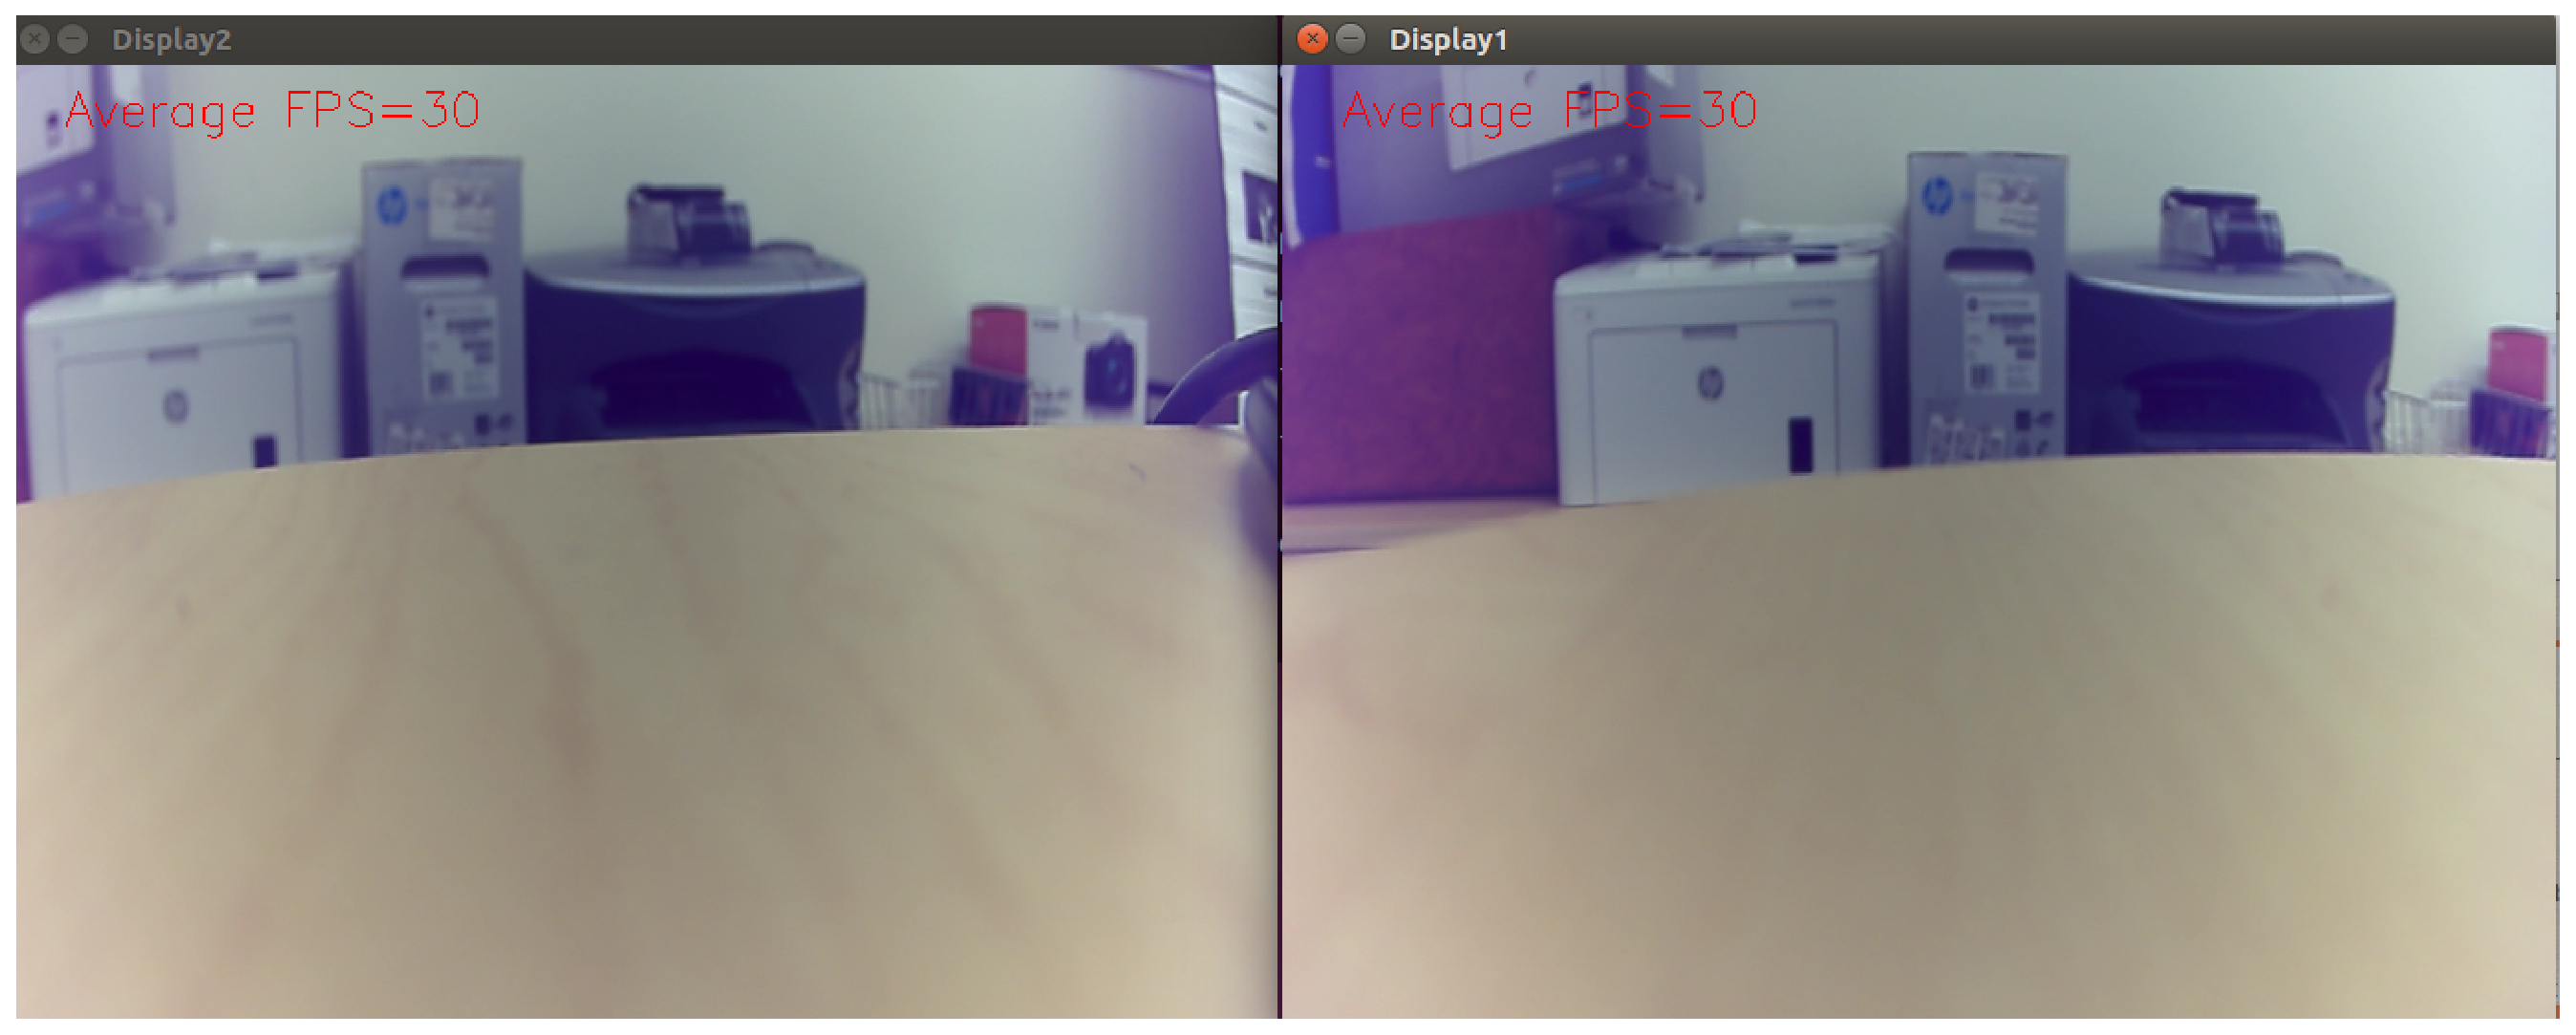
\includegraphics[width=10cm]{images/fps2.eps}
	\caption{TX2 module on the development kit. \label{overflow}}
\end{figure}

%\nocite{*}
\newpage
\bibliographystyle{ieeetr}
\bibliography{SpMPR_Group51}
\end{document}
